% !TEX root =  ../master.tex
\chapter{Konzeption}
Bevor mit der Implementierung gestartet werden kann wird ein Konzept erstellt, welches als Leitfaden für die Implementierung dienen soll.
Ziel ist es ein Entwurf zu konkretisieren, welcher die technischen und grundlegenden Funktionalitäten beschreibt.
Dadurch soll verhindert werden, dass die aufwendige Implementierung fehlschlägt oder mehrfach Änderungen durchgeführt werden müssen, welche den Implementierungsaufwand vergrößern würden.

% TODO: Wasserfall / Agile

\section{Konzeption der Anwendungsarchitektur}

\subsection{Infrastruktur}
Die Grundlage jeder Anwendung ist der Aufbau und die Struktur der Infrastruktur, auf welcher die Anwendung später ausgeführt werden soll.
Aus diesem Grund wird diese als erstes betrachtet.

Webanwendungen werden üblicherweise in einem Client-Server-Modell entwickelt.
% TODO: \autocite{Leff}
Der Client übernimmt dabei sämtliche Funktionalitäten, die das Nutzerinterface betreffen.
Dazu zählt die Visualisierung und die Interaktion mit dem Nutzer.
Der Server kümmert sich hingegen um die Geschäftslogik, Datenhaltung und Datenaustausch.
In \autoref{fig:clientServerAufbau} ist eine solche Architektur vereinfacht dargestellt.

% TODO: Thin-Client

\begin{figure}[h]
    \centering
    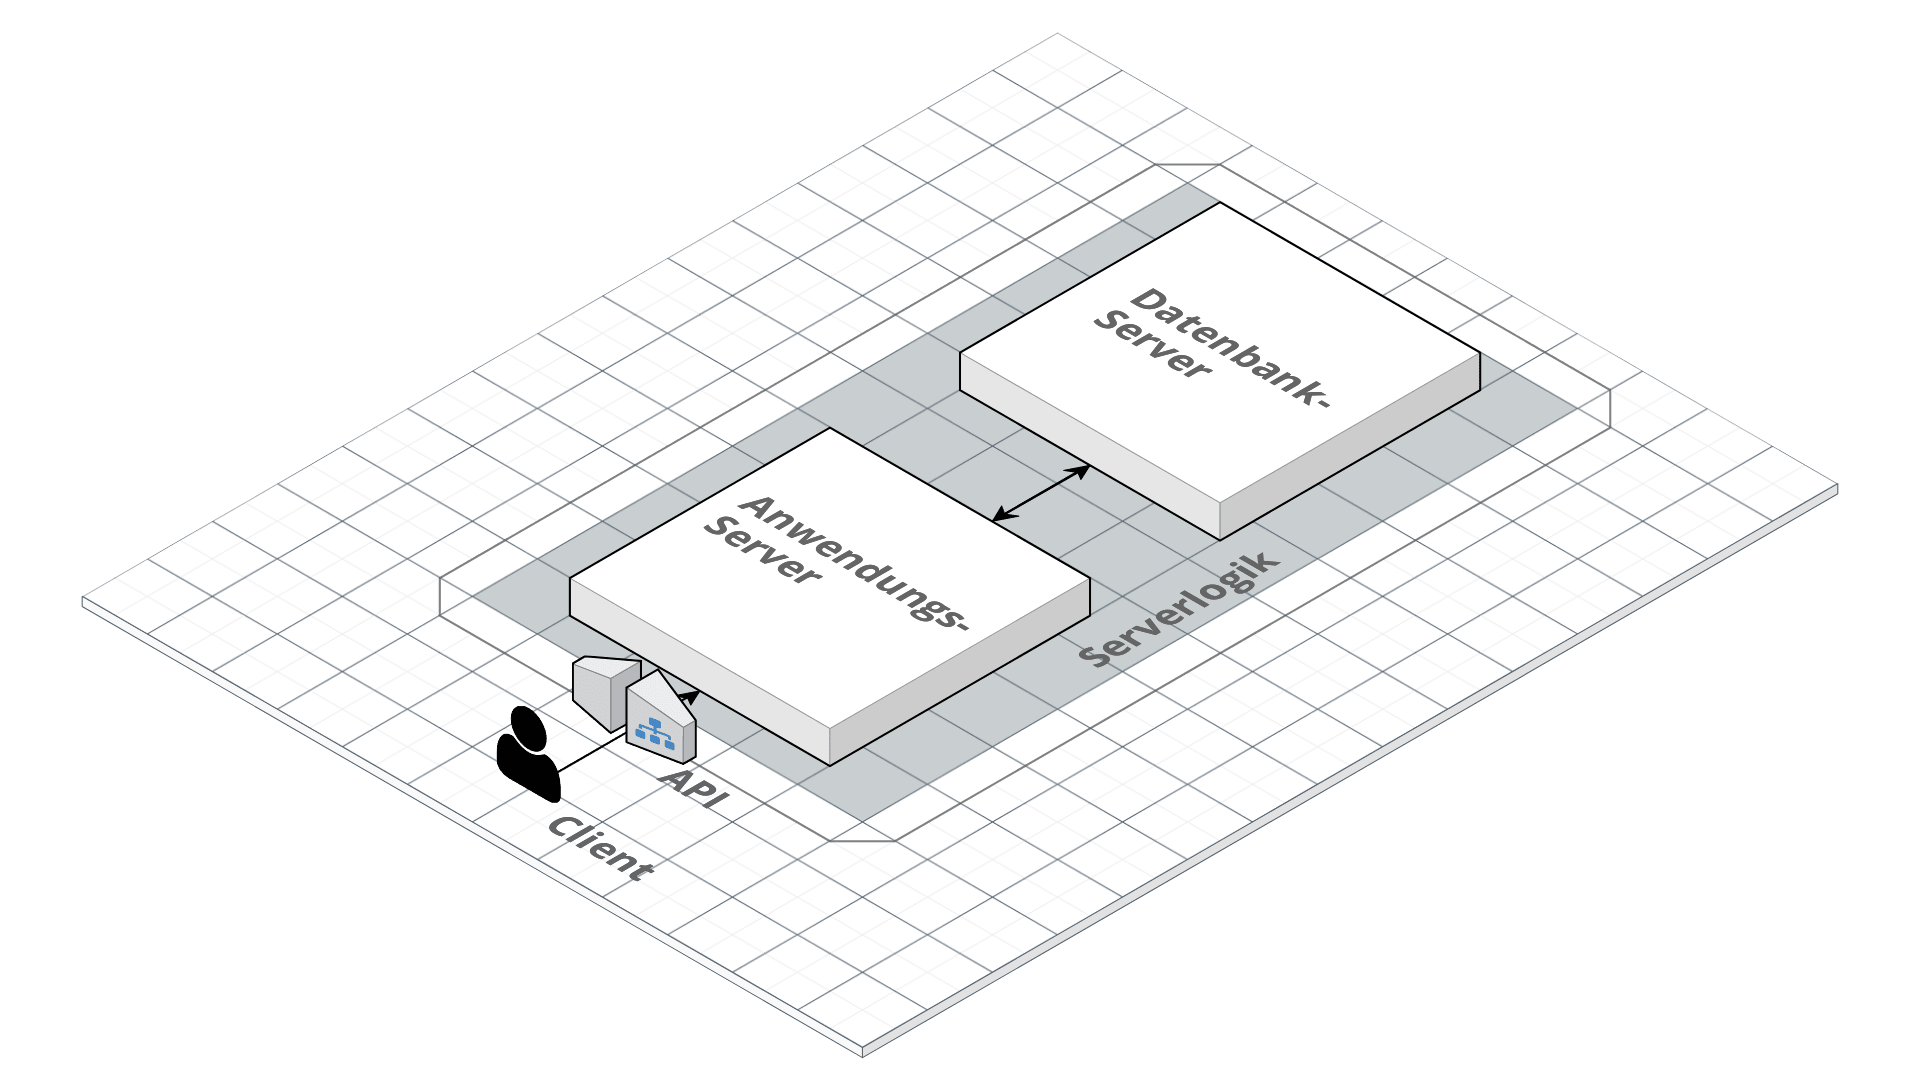
\includegraphics[width=.9\textwidth]{img/ClientServer.png}
    \caption{Vereinfachter Client-Server-Aufbau}
    \label{fig:clientServerAufbau}
\end{figure}

Der Nutzer ruft die mithilfe seines Browsers die Webseite von einem Server ab.
Frägt der Nutzer und in seiner Verlängerung der Browser Daten an, werden diese vom Anwendungsserver geladen.
Dabei greift der Nutzer über eine \ac{API} auf den Anwendungsserver zu.
Dieser läd die notwendigen Informationen auf ähnliche Weise von einem Datenbankserver und bereitet diese gegebenenfalls auf.

Nach den Anforderungen ist eine hohe Leistungsfähigkeit benötigt wird, die auch mit Leistungsspitzen klar kommt.
Der Nachteil von Client-Server-Modellen ist der hohe Aufwand im Bereich der Skalierung.
Das heißt, sobald eine Leistungsspitze entsteht müssen erst aufwändig zusätzliche Server hochgefahren werden, welches die Anwendung kurzzeitig für viele Nutzer unnutzbar macht.
Aus diesem Grund haben wir uns für einen modernen \enquote{Serverless}-Ansatz entschieden.

% TODO: Cloud Computing

% TODO: Serverless Computing
% TODO: Das vielleicht in Grundlagen verschieben
% TODO: Hier kann man noch super viel schreiben

% TODO: Hier noch vielmehr schreiben wie Nutzenanalyse? + viel überleitung


\begin{figure}[h]
    \centering
    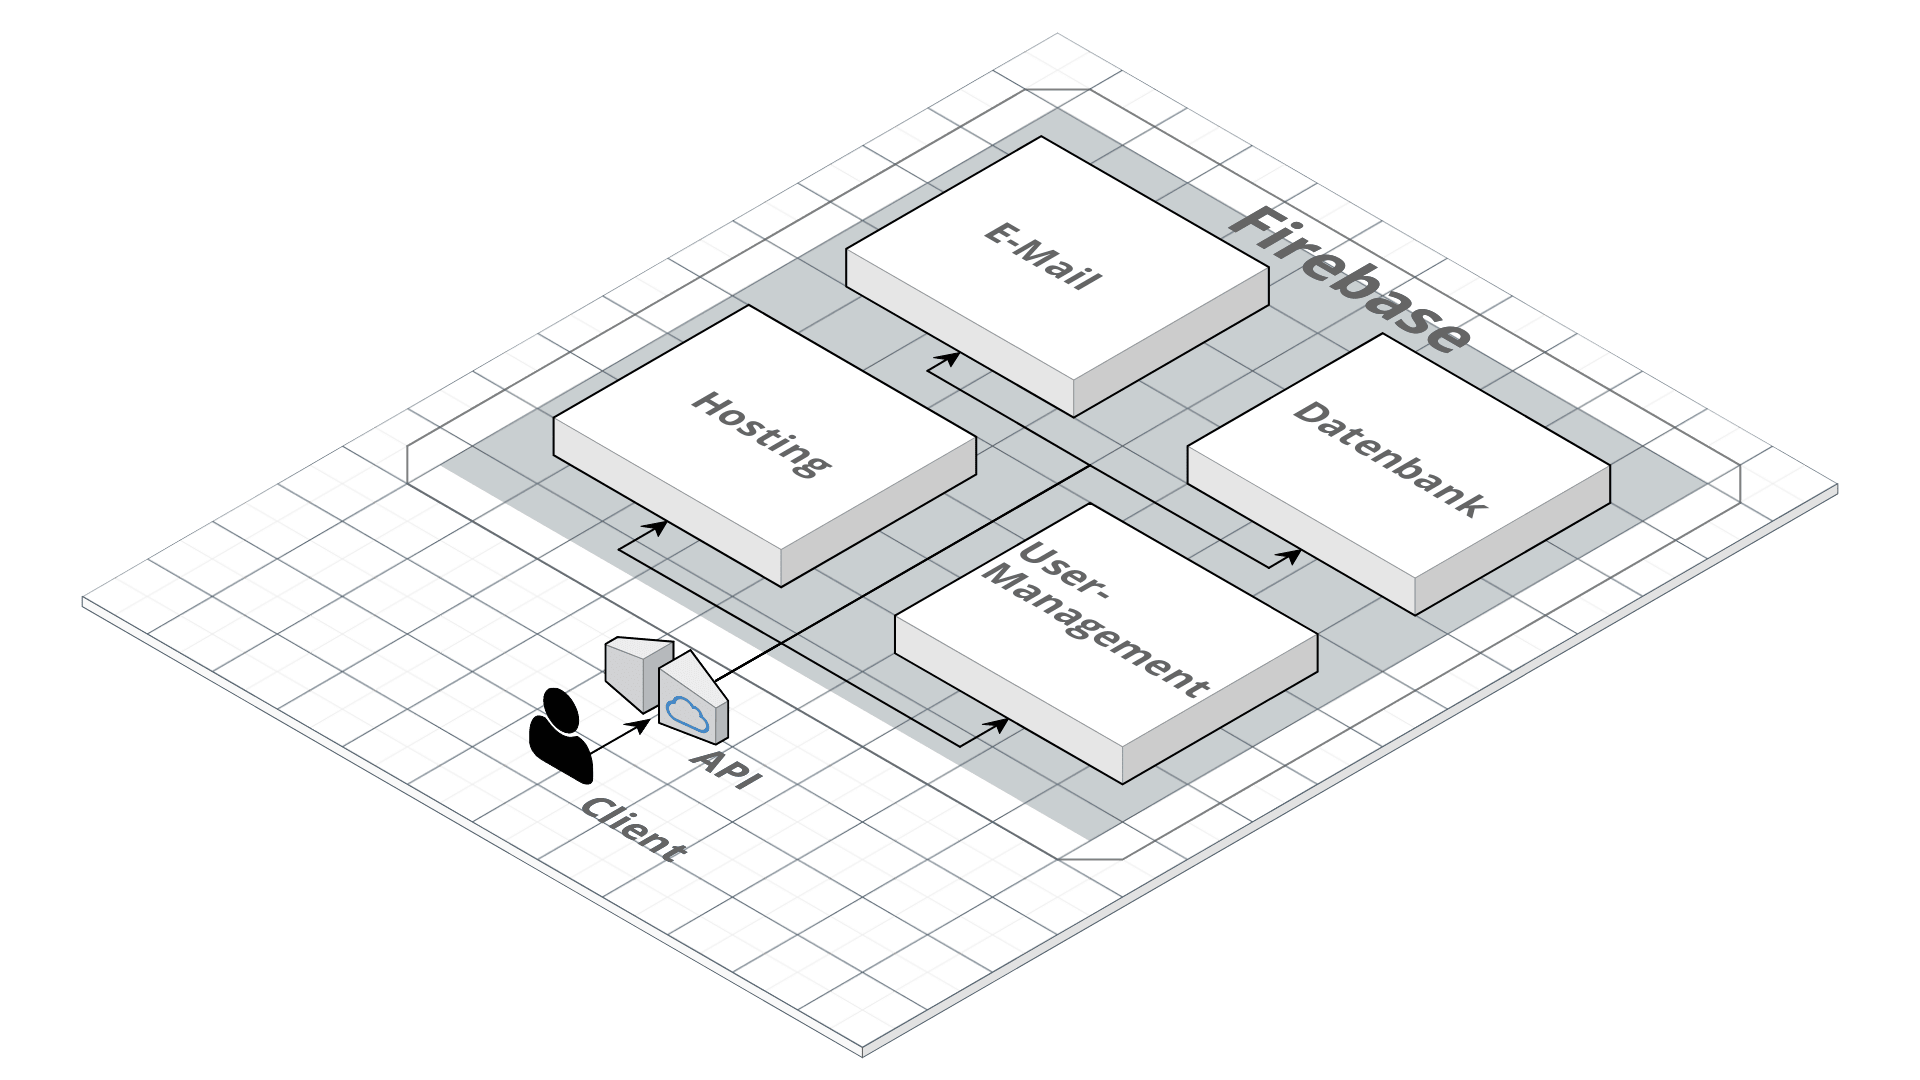
\includegraphics[width=.9\textwidth]{img/Firebase.png}
    \caption{Vereinfachter Firebase-Aufbau}
    \label{fig:firebaseAufbau}
\end{figure}



\subsection{Anwendungsaufbau}
Für das Nutzerinterface werden verschiedene Technologien verwendet.
% Firebase
Die Frontend-Anwendung ist mit Angular, Nebular, Firebase, RxJS ... % TODO: Was muss hier tatsächlich erwähnt werden? Die anderen erzählen ja wirklich aaaallles


Angular ist ein von Google entwickeltes Javascript Framework zur Erstellung interaktiver 



Die Anwendung folgt dem \ac{MVC}-Pattern. Das heißt, die Anwendung ist aufgeteilt in 3 Bereiche:
\begin{itemize}%TODO: Hier kann man noch mehr schreiben
    \item Model\\
        Das Modell stellt den aktuellen Status bzw. den aktuellen Zustand der Anwendung dar.
    \item View\\
        Die Präsentation ist zuständig für die Darstellung der Daten und ermöglicht dem Benutzer die Interaktion mit diesen sowie die Steuerung der Anwendung.
    \item Controller\\
        Der Controller kümmert sich um die Steuerung der Anwendung. Er verwaltet die Präsentation und steuert den Datenfluss zwischen der Präsentation und dem Modell.
\end{itemize}


\section{Konzeption der Funktionalitäten}


\subsection{Kurseinschreibung} %TODO: F2,   das hier vielleicht mit Rollenzuweisung tauschen von der Reihenfolge
Aus den Anforderungen geht hervor, dass es zwei Nutzerrollen gibt: Dozenten und Studenten.
Dozenten sollen in der Anwendung ihre Kurse verwalten können.
Ein Kurs orientiert sich dabei an der Organisation, die in der Realität vorliegen.
Auch in vorhandenen Tools wie beispielsweise \enquote{Moodle} sind Studenten anhand von Kursen organisiert.
Aufgrund der Vielzahl an solchen Lösungen scheint sich eine solche Organisation zu bewähren.
Aus diesem Grund liegt es nahe, das auch die zu entwickelnde Anwendung eine solche Struktur nutzen sollte.
% TODO: Wie Werden Kurse erstellt

Nachdem nun geklärt wurde, wie die Organisation von Studenten und Dozenten stattfindet, muss nun die Zuweisung von Studenten zu Kursen die Zuweisung von Dozenten konzipiert werden.
Zunächst wird die Studentenzuweisung betrachtet.
Für die Zuweisung von Studenten kommen mehrere Ansätze in betracht, die sich in der Person unterscheiden, die die Zuweisung durchführt:
\begin{enumerate}
    \item Zuweisung durch Anwendungsadministrator
    \item Zuweisung durch Dozenten
    \item Zuweisung durch Studenten
\end{enumerate}
Als erster Ansatz kommt die Zuweisung durch einen Anwendungsadministrator in betracht.
Ein solcher Administrator ist ein zentraler Mitarbeiter der DHBW, welcher komplette Autorität über die Anwendung besitzt.
Von einem solchen Ansatz wird abgesehen, da der Verwaltungsaufwand sehr hoch ausfällt.
Für jeden Kurs über 20 Studenten zuzuweisen, und das für mehrere Kurse pro Semester und Vorlesung, scheint nicht realistisch.

Der zweite ist der Ansatz der Zuweisung durch einen Dozenten.
In der aktuellen DHBW-Organisation besitzen Dozenten bereits eine Liste an Studenten für ihre Vorlesung.
Diese Liste dient zur Anwesendheitskontrolle.
Demnach können Dozenten diese Liste für die Zuweisung in der Anwendung nutzen.
Der Nachteil eines solchen Ansatzes ist es aber, dass Studenten ihre Daten in der Anwendung hinterlassen müssen und diese durch andere Dozenten gegebenenfalls einsehbar wären.
Zusätzlich geht die Anonymität, welche durch Matrikelnummern gegeben ist eventuell verloren.
Insgesamt ist dieser Ansatz aus Datenschutzaspekten besonders kritisch. % TODO: Beim Admin nicht so, weil dhbw

Als Letzter Ansatz ist die Zuweisung durch den Studenten.
Denkbar sind hier mehrere Ansätze: Eine Liste aus Kursen oder über einen Kursidentifikator.
Eine Liste mit Kursen vereinfacht die Zuweisung durch den Studenten, da Kurse schnell entdeckt werden können und eventuell zusätzliches Wissen vermittelt werden kann, wenn der Student sich für mehrere ähnliche Kurse einträgt.
Nachteil ist aber die unmittelbare Verwaltung und Übersicht über die Kurse.
Eine Zuweisung über einen Kursidentifikator (kurz: Schlüssel) hat den Nachteil, dass diese Schlüssel erst aufwändig über einen weiteren Kommunikationsweg (z.\,B. Email oder direkt in einer Vorlesung) mitgeteilt werden muss.
Dafür besitzen Studenten aber nur Zugriff auf die für sie relevanten Vorlesungen.
In \enquote{Moodle} ist die Zuweisung zu Kursen auf freiwilliger Basis anhand von Einschreibeschlüsseln gelöst.
Aus diesem Grund ist dieser \enquote{Workflow} bereits für Studenten bekannt und eine Anpassung an die neue Anwendung ist schnell möglich.
In der Tat nutzen viele existierende Anwendungen ein solches System.
Beispiele hierfür sind Zoom oder Google Meets.

% TODO: Bei uns:
Ein Einschreibeschlüssel besteht aus 6 Buchstaben, welche mehr als 300 Millionen Kurse zulassen und als ausreichend angesehen werden.


\subsection{Rollenzuweisung} %TODO: Nochmal auf die Anforderungen F7 verweisen
Nutzer der Anwendung können sich selbst registrieren.
Daraus ergibt sich die eine Rollen Problematik: Woran kann die Anwendung erkennen, welcher Nutzer ein Student ist und welcher Nutzer ein Dozent ist.
Sofern Nutzer dies selber angeben können, bräuchte es gegebenenfalls eine Validierung durch die DHBW, wodurch erneut die oben genannten Nachteile einer Zuweisung durch einen Administrator greifen.
Ein Ansatz, bei dem Nutzer dies selber verwalten können wird auch hier als besser angesehen.
Aus diesem Grund wird der folgende Ansatz verwendet:
Statt festdefinierte Rollen (Student und Dozent) zu besitzen, kann jeder Student selbst sowohl Student, als auch Dozent sein.

Jeder Nutzer ist zunächst keiner Rolle zugeordnet.
Jeder Nutzer kann einen Kurs erstellen, wodurch dieser Nutzer automatisch zu einem Dozent für diesen Kurse.
Sobald sich ein Nutzer mithilfe des Einschreibeschlüssels für einen Kurs anmeldet wird der Nutzer automatisch für diesen Kurs zu einem Studenten.
Dadurch können auch zuvor nicht vorgesehene Nutzerbeziehungen entstehen.
Beispielsweise kann ein Dozent sich in einen weiteren Kurs einschreiben, falls er sich in einer weiteren Richtung weiterbilden möchte.
Oder die DHBW kann sich in für einen Kurs einschreiben um die Qualität einer Vorlesung zu validieren.


Ein Vorteil eines solchen Ansatzes ist es, dass auch Studenten Kurse erstellen können und so Lerngruppen gefördert werden.
Denkbar ist beispielsweise ein Student, welcher Nachhilfe anbietet.
Dadurch wird die Nutzung der Anwendung gefördert.



% TODO: Mocks und alles

% \section{Frontendarchitektur}



% TODO: ER-Modell

\section{Datenstruktur} % TODO: Das nach den Funktionen hinschreiben
In \autoref{fig:erDiagramm} ist das zugrundeliegende Datenmodell abgebildet, welches in der Implementierung verwendet wird.

\begin{figure}[h]%FIXME: Das hier erweitern, wenn alle Daten drin sind + das watermark abschneiden
    \begin{center}
        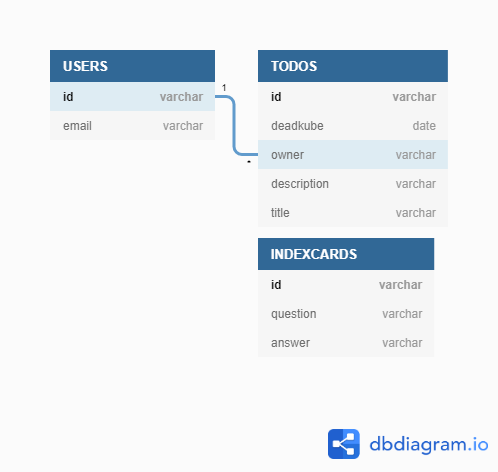
\includegraphics[width=.7\textwidth]{img/Integrationsseminar ER.png}
        \caption{ER-Diagramm}
        \label{fig:erDiagramm}
    \end{center}
\end{figure}

Die Datenspeicherung findet vollständig innerhalb von Firebase statt.
Der hierfür genutzte Service heißt \enquote{Firestore}.
Dabei werden Daten nicht wie in einer klassischen relationalen Datenbank (\ac{RDB}) in Tabellen mit Spalten und Zeilen gespeichert, sondern in Collections aus Dokumenten.





% \subsection{Studierende}
% \subsection{Dozierende}
% \subsection{Kurs erstellen}
% \subsection{Karteikarten-Lernsystem}
% \subsection{ToDo-Liste}
% \section{Datensicherheit}
% \section{Datenschutz}
% \section{Grundlage für Datenauswertung}
% % Hier Verweise auf Aubau und Bezug zum leichten Ausbau, etc.








\section{Ich mach hier einen WIP Abschnitt :D}




% TODO: Das besser mit den Anforderungen verknüpfen
% TODO: Dokumentation über TODOS


% TODO: Todos und index-cards auch löschbar und alles

% TODO: Wie technisch?






% TODO: Dokumentation über Authentifizierung
% TODO: Dokumentation über Index-Cards
% TODO: Screenshots
% TODO: Aria?





% Ein Dozent sollte dabei beispielshaft einen Kurs anlegen können







% TODO: Caching


% TODO: Lighthouse am schluss beschreiben, wenn wir alle unnötigen Abhängigkeiten entfernt haben?

% TODO: Kann man nach offline machen?

Der Ladefortschritt kann stets an der Leiste am oberen Bildschirmrand abgelesen werden.


% TODO: Offline erwähnen + Anforderungen

\section{Offline Synchronisation}
Studenten sind oft unterwegs beispielsweise in öffentlichen Verkehrsmitteln, in dehnen Internet nicht immer verfügbar ist.
Damit die Anwendung auch ohne Internet funktionsfähig ist, ist die Anwendung mit einer Offline-Synchronisation ausgestattet.

Sobald sich der Nutzer angemeldet hat, kann die Anwendung vollständig offline genutzt werden.
Sobald eine Internetverbindung besteht werden alle Änderungen synchronisiert.

Sofern die Anwendung offline gleichzeitig auf mehreren Geräten mit dem gleichen Nutzer verwendet wurde können bei Datenspeicherungen Konflikte auftreten.
Solche Konflikte werden nach dem Last-Write-Wins-Prinzip aufgelöst.
Das heißt die letzte Änderung an einem Datensatz wird übernommen.
% TODO: IndexDB


\section{DevOps}
Für die Entwicklung und der Betrieb werden üblicherweiße viele verschiedene Parteien benötigt.
Beispielsweise werden Entwickler, Administratoren und Netzwertechniker benötigt.
Durch den Einsatz von DevOps-Praktiken ändert sich die Art und Weise wie Anwendungen entwickelt werden.

DevOps verbindet die beiden Bereiche \enquote{Development} und \enquote{Operations}.
Ziel ist es, die Entwicklung und den Betrieb von Softwaresystemen zu kombinieren und so den Organisationsaufwand sowie die Zeit zwischen Auslieferungszeitpunkten zu minimieren.\autocite[][S. 156]{Artac2018}

Im Rahmen von DevOps-Prozessen werden üblicherweiße \ac{CI}- und \ac{CD}-Pipelines erstellt, welche die Bereitstellung einer Anwendung automatisieren.
So wurde im Rahmen der hier entwickelten Anwendung eine automatisierte Deployment-Strategie ausgearbeitet.

% TODO: Github erwähnen?
% TODO: Changelog?
Sobald ein Release erstellt wird, beginnen automatisch Pipelines.
Diese bauen die Anwendung und stellen diese anschließend auf der Infrastruktur bereit, sodass dies von Anwendern genutzt werden kann.
Die Bereitstellung findet dabei Unterbrechungsfrei statt.
Bei klassischen Anwendungen müssen im Regelfall Wartungsarbeiten angekündigt werden und die Anwendungen sind währenddessen nicht nutzbar.
In der hier entwickelten Anwendung ist dies hingegen nicht notwendig.
Auch während eine neue Version bereitgestellt wird ist die Anwendung dauerhaft nutzbar.

Gleichzeitig wird als Teil der Pipelines die Dokumentation erstellt.

Durch die Pipelines können Deployments mit wenigen Klicks von jedem Computer oder Mobilgerät durchgeführt werden, egal wo oder welches System genutzt wird.
Gleichzeitig ist stets dokumentiert wann und von wem welche Version bereitgestellt wurde.







\section{Performance Optimierungen}
% TODO: Irgendwo hab ich ja schon gesagt, das firebase spitzenlasten abfängt
\subsection{Caching}
In der Anwendung werden aus verschiedenen Gründen Caching eingesetzt.
Caching beschreibt eine Methode, bei dem Daten in einem Puffer gehalten werden um Zugriffe auf langsame Ressourcen zu reduzieren.
Im Falle der hier entwickelten Anwendung werden die Quelldaten für das Nutzerinterface lokal aufbewahrt um die Zugriffe auf den Server zu reduzieren.
Dadurch wird die Ladezeit der Anwendung reduziert, mobile Daten gespart und die Serverlast reduziert.


% \section{Verschlüsselung}
% TODO:

% Kompression

% h2 protokol


\subsection{Service-Worker}
% Vielleicht kann sowas sagen wie: Wir haben weniger funktionalität, dafür läuft alles stabil und ist schon bereitgestellt + Technik generell viel besser
Die Anwendung ist mit einem Service-Worker ausgestattet.
Der Service-Worker agiert als Zwischeninstanz zwischen der Webanwendung und dem Server.
Durch den Service-Worker ist es möglich die Website als eigene Anwendung auf einem Mobilgerät oder auf Desktop-Computern installiert werden kann.
Dadurch kann die Anwendung wie jede andere App verwendet werden.



\subsection{Lazy Loading}
Die Anwendung unterstützt Code-Splitting mit Lazy-Loading.
Das bedeutet, die Anwendung ist modular aufgebaut und wird zum Zeitpunkt der Bereitstellung automatisch in verschiedene Module aufgespalten.
Besucht der Nutzer die Website der Anwendung werden nur die Teile der Anwendung heruntergeladen, die für ihn tatsächlich notwenig sind.
Beispielsweise werden die Karteikarten, sowie die gesamte Funktionalität und Darstellung dieser nicht geladen, wenn der Nutzer nur seine Todos nachschaut.


\section{Datenschutz}
Bei der Entwicklung der Anwendung haben wir großen Wert auf Datensicherheit und der Einhaltung der DSGVO gelegt.
Ein wesentlicher Bestandteil der unternommenen Maßnahmen ist die Anonymität innerhalb der Anwendung.
Die Anwendung speichert keinerlei Informationen, worüber Nutzer identifiziert werden können.
Bei einer Registrierung muss lediglich eine Email angegeben werden.





\section{Personas}


% -------------------------------------------------------
% 1. Student
% 2. Dozent
% -------------------------------------------------------
% Keine Ahnung, irgendwelche Bilder halt :D
% TODO: Das ist noch sehr kopiert

% https://unsplash.com/photos/ZVo7vtXilCs
\subsection{Beispiel Persona für Student}

\begin{minipage}[t]{0.5\textwidth}
	\vspace{-4cm}
	\renewcommand{\arraystretch}{1.5}
	\begin{tabular}{l l}
		Name: & Stephan Student \\
		Alter: & 21 \\
		Tätigkeit: & Student Wirtschaftsinformatik \\
		IT-Skills: & 4/5 \hspace{-1cm} \begin{barchart}{5.0}
			\baritemNL{}{4}
		\end{barchart} \\
	\end{tabular}
\end{minipage}
\hfill
\begin{minipage}[t]{0.4\textwidth}
	\flushright
	
\includegraphics[width=0.70\textwidth]{img/carlos-lindner-ZVo7vtXilCs-unsplash.jpg}
\end{minipage}


Stephan ist ein typisches Beispiel für einen Studenten an der DHBW.
Er ist viel aktiv und war in der Vor-Corona-Zeit eine Person, die zur DHBW gependelt ist.
Demnach möchte er egal wo er ist stets eine Übersicht über seine anstehenden Klausuren haben und sich auch unterwegs auf diese Vorbereiten.
Dabei ist es ihm wichtig, dass seine persönlichen Daten nicht Weitergegeben werden und nicht zur Klausurbewertung oder Ähnliches herangezogen werden können.

Das möchte ich gerne haben:
\begin{itemize}
	\item Übersicht über meine Klausuren
	\item Auch unterwegs lernen können
	\item Anonymität
\end{itemize}


\clearpage
\subsection{Beispiel Persona für Dozent}
% https://unsplash.com/photos/TXxiFuQLBKQ
\begin{minipage}[t]{0.5\textwidth}
	\vspace{-4cm}
	\renewcommand{\arraystretch}{1.5}
	\begin{tabular}{l l}
		Name: & Dagmar Dozent \\
		Alter: & 35 \\
		Tätigkeit: & Dozentin für Finanzbuchhaltung \\
		IT-Skills: & 2/5 \hspace{-1cm} \begin{barchart}{5.0}
			\baritemNL{}{4}
		\end{barchart} \\
	\end{tabular}
\end{minipage}
\hfill
\begin{minipage}[t]{0.4\textwidth}
	\flushright
	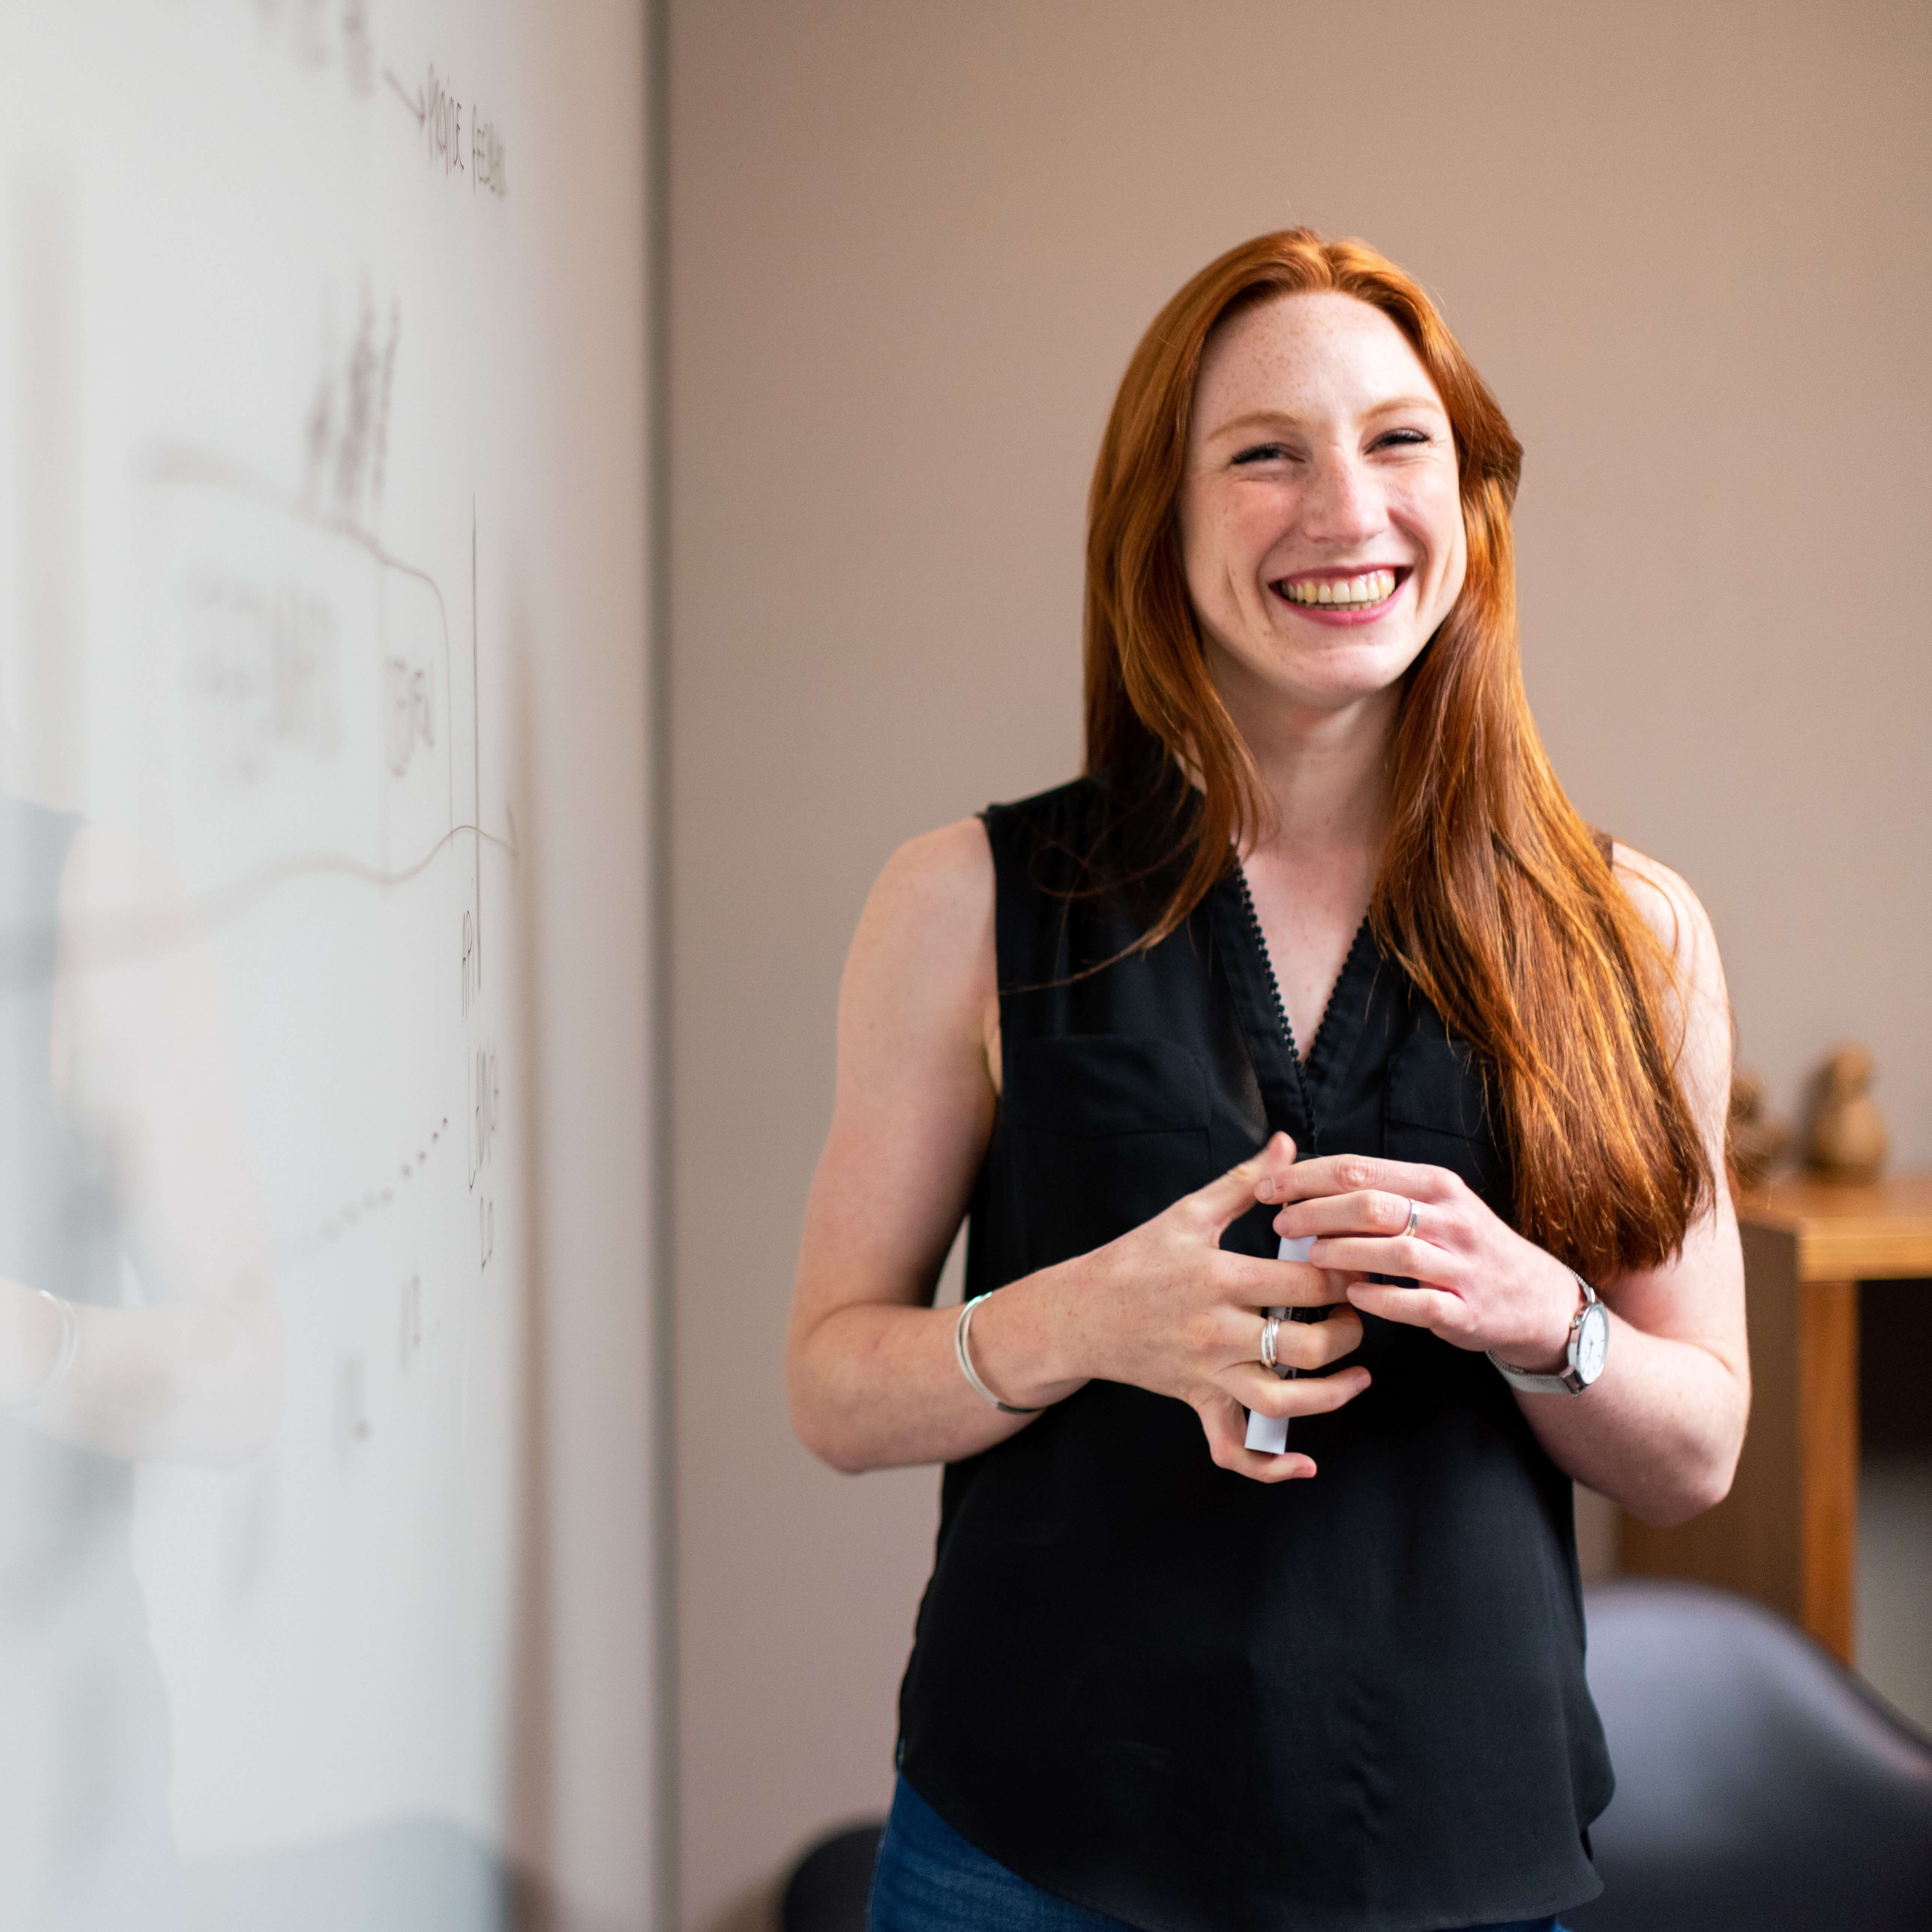
\includegraphics[width=0.70\textwidth]{img/thisisengineering-raeng-TXxiFuQLBKQ-unsplash.jpg}
\end{minipage}

Dagmar ist eine Dozentin für Wirtschaftsthemen, vorrangig Finanzbuchhaltung.
Als verantwortungsbewusste Person ist es ihr wichtig, dass Studenten auch außerhalb ihrer Vorlesung Unterstützung erhalten.
Aus diesem Grund möchte sie gerne weiterführende Informationen an Studenten weitergeben.
Gleichzeitig möchte sie gerne Feedback zu ihrer Vorlesung erhalten um das Lernmaterial bestmöglich anzupassen.
Da sich allerdings ihre Kernkompetenzen außerhalb der IT befinden ist es ihr wichtig, dass sie die Anwendung nutzen kann ohne eine lange Einführung erhalten zu müssen. 


Das möchte ich gerne haben:
\begin{itemize}
	\item Informationen an alle Studenten des Kurses verteilen
    \item Feedback zum Kurs erhalten %TODO: Sowas noch implementieren
    \item Intuitives Interface
\end{itemize}

